\documentclass[tikz,border=0pt]{standalone}
\usepackage[american]{circuitikz}
\usetikzlibrary{arrows.meta,calc,positioning,decorations.pathmorphing,patterns}
\definecolor{zyloTeal}{HTML}{174A5B}
\definecolor{zyloTealTwo}{HTML}{246B7A}
\definecolor{zyloInk}{HTML}{1F2933}
\definecolor{zyloSoft}{HTML}{EAF4F4}
\definecolor{zyloPaper}{HTML}{F8FAFB}
\definecolor{zyloLine}{HTML}{44606B}
\definecolor{zyloOrange}{HTML}{D97706}
\begin{document}
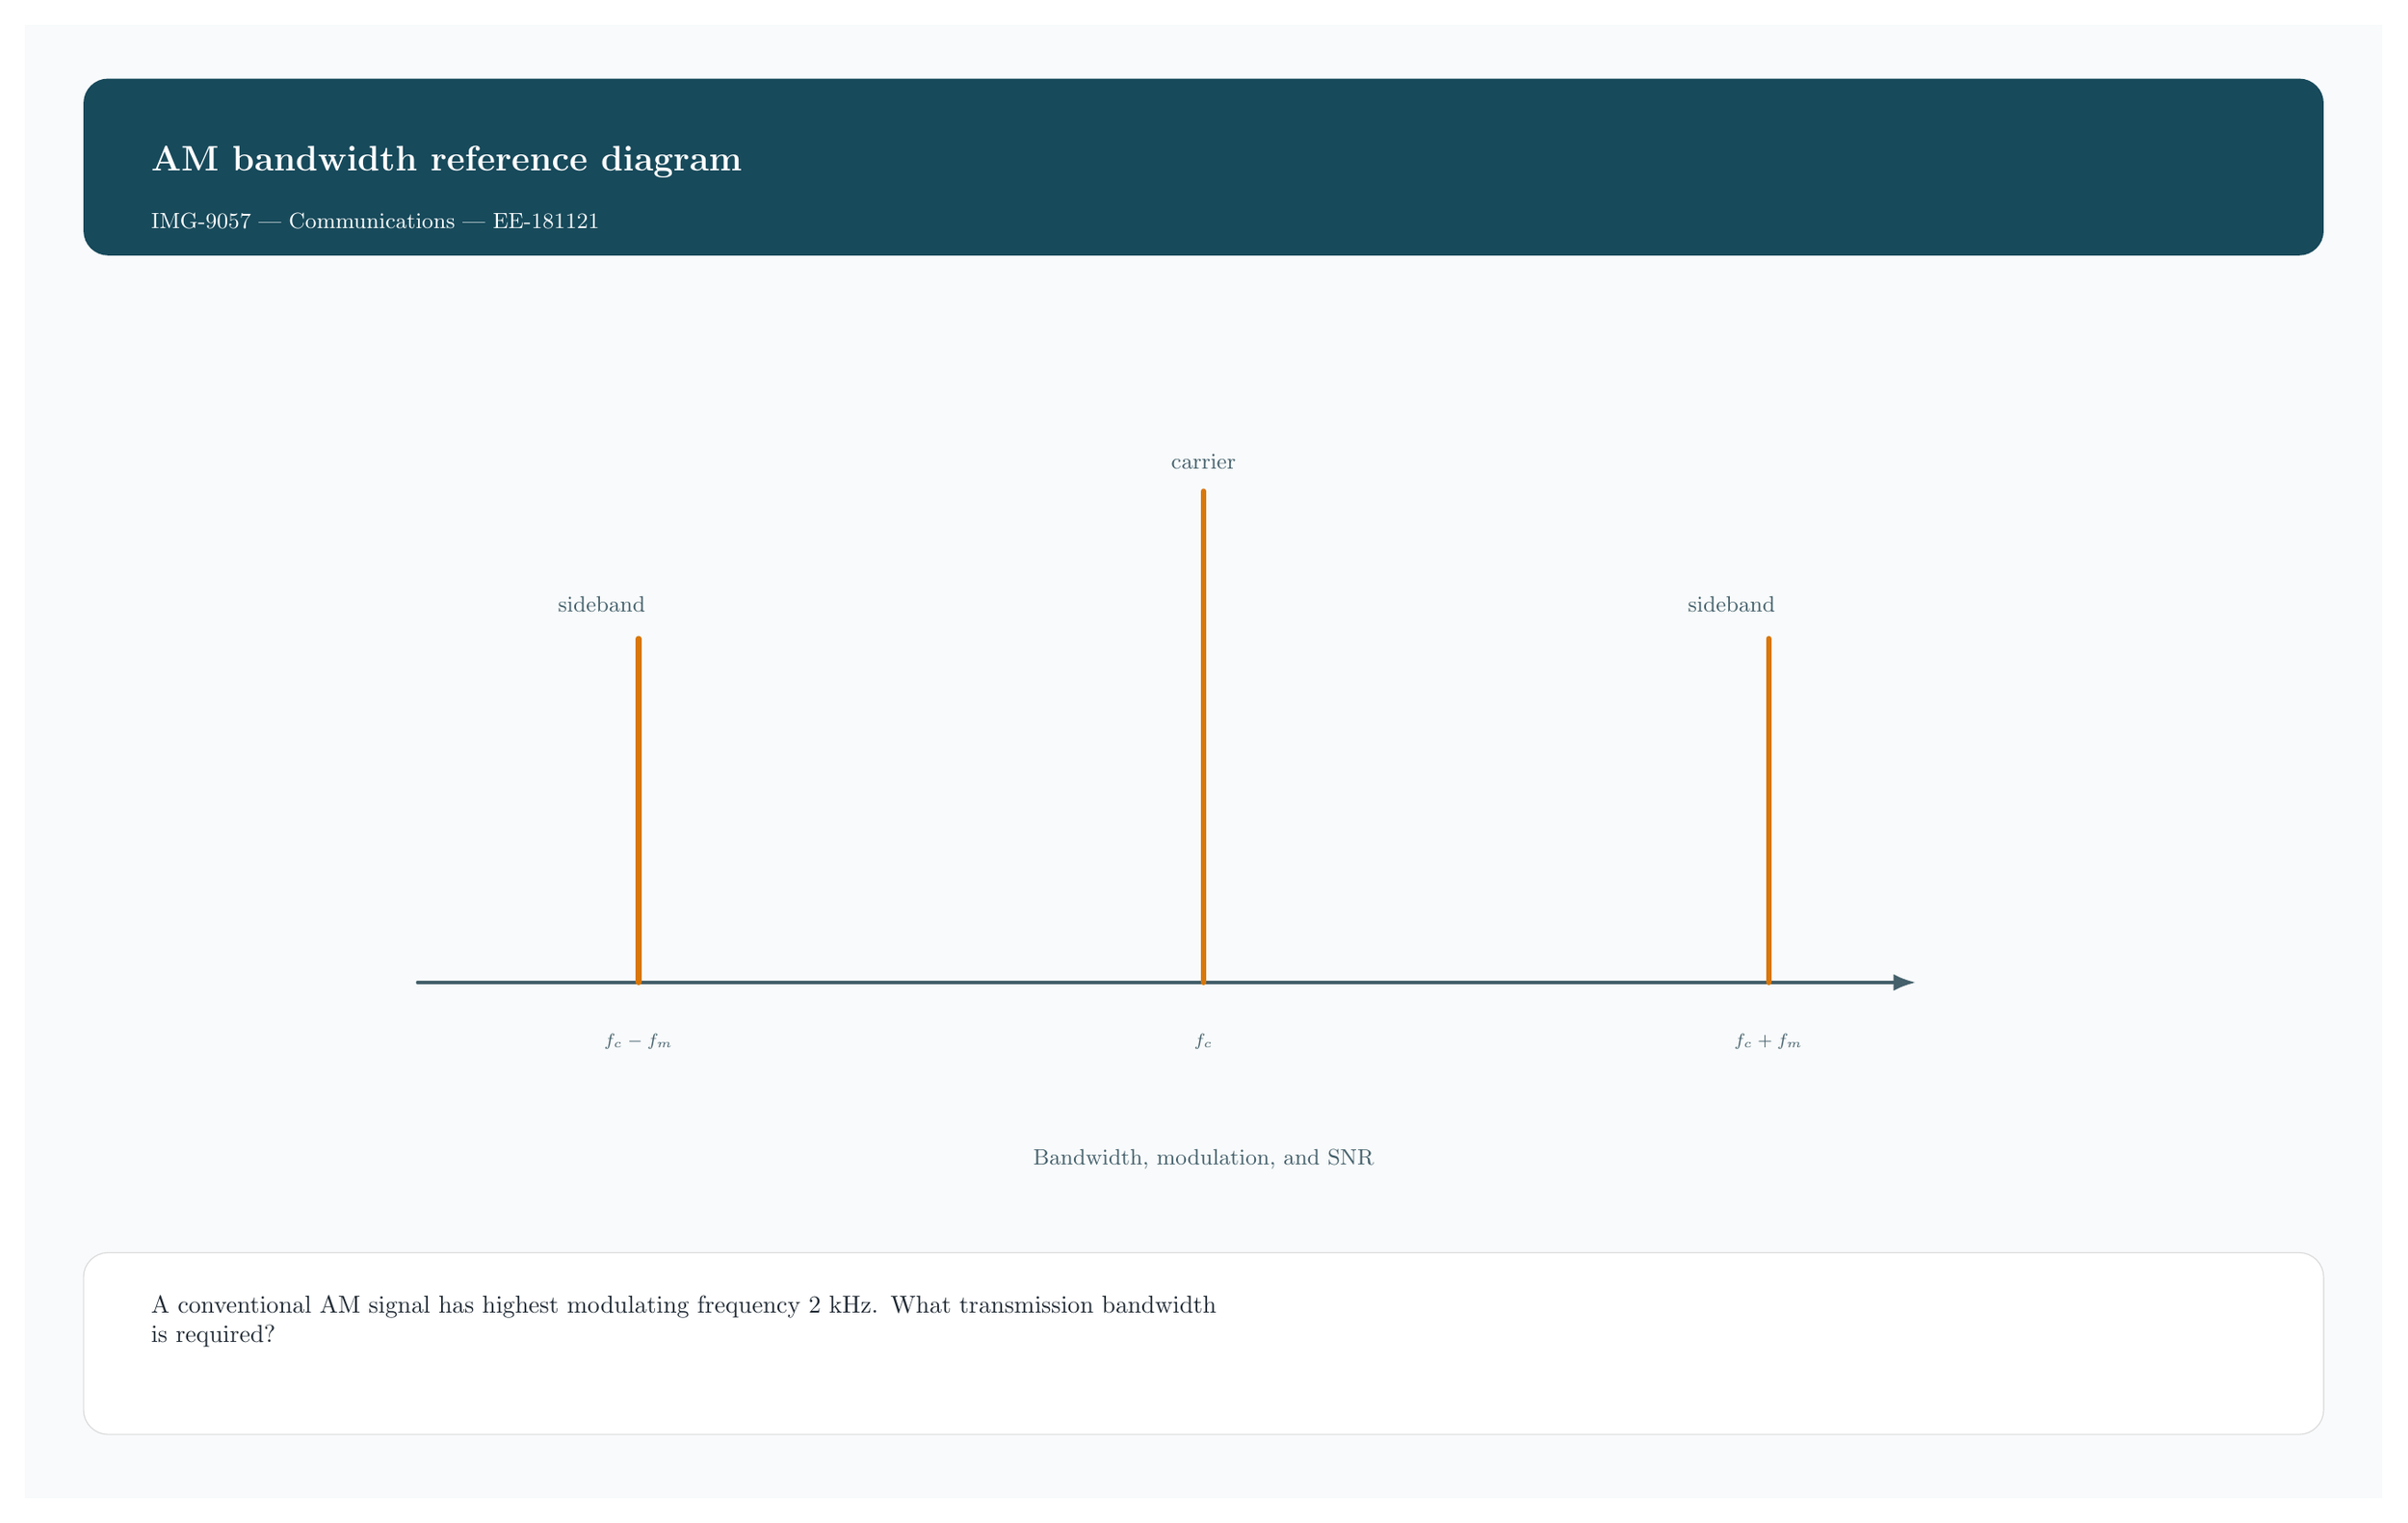
\begin{tikzpicture}[x=1pt,y=-1pt,>=Latex,line cap=round,line join=round]
\path[fill=zyloPaper] (0,0) rectangle (960,600);
\path[fill=zyloTeal,rounded corners=10pt] (24,22) rectangle (936,94);
\node[anchor=west,text=white,font=\bfseries\Large] at (48,56) {AM bandwidth reference diagram};
\node[anchor=west,text=white!82,font=\small] at (48,80) {IMG-9057 | Communications | EE-181121};
\tikzset{wire/.style={draw=zyloTeal,line width=2.2pt},thinwire/.style={draw=zyloLine,line width=1.35pt},accent/.style={draw=zyloOrange,line width=2.2pt},box/.style={draw=zyloTealTwo,fill=zyloSoft,line width=1.5pt,rounded corners=8pt}}
\draw[thinwire,->] (160,390) -- (770,390);
\draw[accent] (250,390) -- (250,250); \draw[accent] (480,390) -- (480,190); \draw[accent] (710,390) -- (710,250);
\node[font=\scriptsize,text=zyloLine] at (250,414) {$f_c-f_m$}; \node[font=\scriptsize,text=zyloLine] at (480,414) {$f_c$}; \node[font=\scriptsize,text=zyloLine] at (710,414) {$f_c+f_m$};
\node[font=\small,text=zyloLine] at (480,178) {carrier}; \node[font=\small,text=zyloLine] at (235,236) {sideband}; \node[font=\small,text=zyloLine] at (695,236) {sideband};
\node[font=\small,text=zyloLine] at (480,462) {Bandwidth, modulation, and SNR};
\path[draw=black!15,fill=white,rounded corners=10pt] (24,500) rectangle (936,574);
\node[anchor=west,text width=860pt,align=left,text=zyloInk,font=\normalsize] at (48,528) {A conventional AM signal has highest modulating frequency 2 kHz. What transmission bandwidth\\is required?};
\end{tikzpicture}
\end{document}
